\documentclass[11pt,a4paper]{article}
\usepackage[margin=1in]{geometry}
\usepackage{url}
\usepackage{hyperref}
\usepackage{paralist} % For use with \begin{compactitem}... or \begin{compactenum}
\usepackage{microtype}		% For decreasing the hyphenation frequency
\microtypesetup{activate=true}
\usepackage{xcolor}
\usepackage{placeins}
\usepackage{graphicx}

\makeatletter
\def\ps@pprintTitle{%
  \let\@oddhead\@empty
  \let\@evenhead\@empty
  \def\@oddfoot{\reset@font\hfil\thepage\hfil}
  \let\@evenfoot\@oddfoot
}
\makeatother


\begin{document}
%\begin{frontmatter}

\begin{titlepage}
	\clearpage\thispagestyle{empty}
	\centering
	\vspace{1cm}
		
	\rule{\linewidth}{1mm} \\[0.5cm]
	{ \Large \bfseries ISyE 6740 - Summer 2023\\[0.2cm]
		Project Report}\\[0.5cm]
	\rule{\linewidth}{1mm} \\[1cm]

		\begin{tabular}{l p{5cm}}
		\textbf{Team Member Names:} \\Vivi Banh (Proposal, Final Report, and Model Evaluation) \& Chukwuemeka Okoli (Proposal, Final Report, and Model Development) \\[10pt]
		\textbf{Project Title:} \\Deep Neural Network for Shoe Model Identification  \\[10pt]
		%\textbf{Please include (at least) the following sections.} & \\
		\end{tabular} 

\end{titlepage}	
%\end{frontmatter}
	

\section{Problem Statement}\label{sec1}
In today's fashion-forward society, social media plays a pivotal role in shaping consumer habits and driving trends. As people browse through fashion photos online, they seek convenient ways to identify and purchase the products showcased in those images. However, traditional methods of searching for unknown products on search engines can be frustrating and time-consuming.  \\

\noindent
To address this challenge, our project aims to develop an advanced image classification system specifically designed for identifying shoe classes worn by models in fashion images. Our system will provide users with the specific shoe classes they are interested in accurately recognizing the shoe from an image. If implemented in a production environment with specific business use cases, this streamlined approach can significantly enhance the shopping experience, allowing consumers to easily find and purchase their desired shoe models.\\

\noindent
Integrating our image classification system into popular platforms like Instagram or a web application can bring significant benefits to retailers and e-commerce platforms. By seamlessly incorporating a product identification feature, businesses can captivate potential buyers, enhance customer engagement, and drive conversions. This transformative capability bridges the gap between inspiration and purchase, transforming social media platforms into highly effective sales channels. The integration of our image classification system can create new opportunities for both retailers and consumers, maximizing sales potential and delivering an exceptional shopping experience. 
	
\section{Data Source} 
The data utilized for this project is the UT Zappos50K Shoe Dataset (ver 1.2), curated by Yu and Grauman (2014) and available on Kaggle.com. This comprehensive shoe dataset comprises 50,025 catalog images obtained from Zappos.com. The images have dimensions of 136 x 102 pixels, showcasing shoes centered on a white background and consistently oriented for ease of analysis. The dataset encompasses various shoe models. The classes to predict include 20 different class of shoes. We trained a neural network and evaluate the performance of our trained model.  
		
\section{Methodology} 
Our problem is a classification problem since we are trying to determine the category of shoe or class of shoe from an image of several shoes from different brand names. We utilized a Convolutional Neural Network (CNN) model, a deep learning architecture well-suited for image classification tasks. The CNN model is trained using the labeled shoe images to learn the distinctive features of each shoe model. We built a custom Convolutional Neural Network (CNN) architecture with three convolutional blocks, followed by a classifier head with two dense layers as the starting model. The model uses the Keras Sequential API to create the architecture.

\subsection{Data Preprocessing}
The preprocessing steps we applied including resizing and normalization, to ensure they are in a suitable format for training. Data augmentation techniques such as vertical and horizontal reflections, rotation up to 90 degrees, and vertical and horizontal shifting of the images up to 20\% of their original size will be applied to enhance the model's ability to generalize.  To preprocess the image, we used the MobileNet V2 preprocessing function from Keras API.  To load the images from disk in small batches of size 32, we used an ``ImageDataGenerator``.  We resized the images and used a small images of size 224 * 224. We have 20 classes namely ``Ankle Boots'', ``Knee High Boots'', ``Over the Knee Boots'', ``Prewalker Boots'', ``Mid-Calf Boots'', ``Athletic Sandals'', ``Flat Sandals'', ``Heel Sandals'', ``Boat Shoes'', ``Flats Shoes'', ``Oxfords Shoes'', ``Clogs and Mules Shoes'',  ``Firstwalker Shoes'', ``Sneakers and Athletic Shoes'', ``Heels Shoes'', ``Prewalker Shoes'', ``Crib Shoes'', ``Loafers Shoes'', ``Slipper Heels Slippers'', ``Slipper Flats Slippers'', ``Boot Slippers''. The generator used the folder structure where the images were stored to infer the labels for the images. We split the data into training, validation and testing sets with 70\% of the data for training the model, 15\% for validating the datasetand selecting the best parameters, and 15\% for testing the model. 

\subsection{Model Architecture}
The neural network is organized in layers meaning we take an image of a shoe, pass it through all the layers and get a prediction of what class the shoe belongs too. We used a custom CNN architecture with three convolutional blocks, followed by a classifier head with two dense layers. The convolutional layer consists of many filters giving us multiple feature maps for each filter.  The output of one convolutional layer is used as input into the next layer. The structure of the neural network is shown in \textbf{Fig. \ref{neural_network}} below:

 \begin{figure}[h!]
\centering
  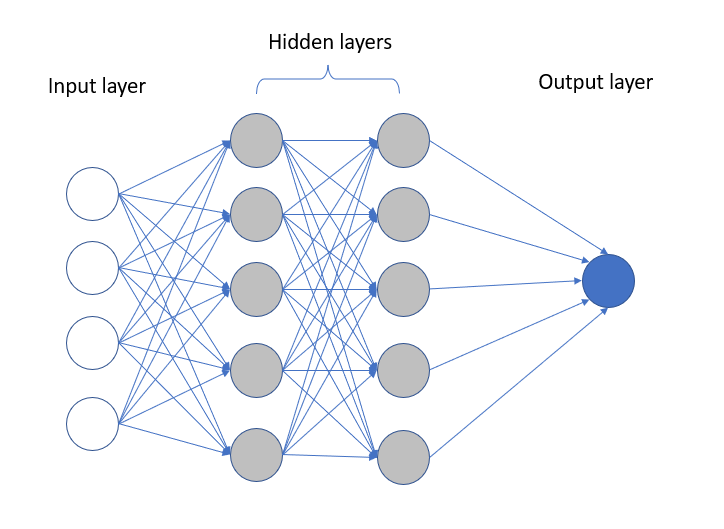
\includegraphics[width=0.75\linewidth]{neural network.png}
  \caption{Structure of a Neural Network}
  \label{neural_network}
\end{figure}

\subsection{Model Development}
The Convolutional Neural Network (CNN) model is designed to process labeled shoe images as input and predict their corresponding shoe model names as target labels. The model's architecture is structured to capture the visual patterns and features associated with each shoe model during the training process.

The model starts with an input layer, utilizing the \emph{Conv2D} layer with the first convolutional block. The first block consists of 32 filters with a kernel size of 5x5, and a \emph{ReLU} activation function is applied to introduce non-linearity. This is followed by a \emph{MaxPooling2D} layer, which performs max-pooling to reduce the spatial dimensions of the output. The second convolutional block is similar to the first, but now with 64 filters and a smaller kernel size of 3x3. After this block, another \emph{MaxPooling2D} layer is applied to further reduce spatial dimensions. The third convolutional block follows a similar pattern, with 128 filters and a kernel size of 3x3. Once again, a \emph{MaxPooling2D} layer is added to reduce the spatial dimensions. After the last \emph{MaxPooling2D} layer, a \emph{Flatten} layer is used to convert the 2D feature maps into a 1D vector. This flattened vector is then passed through the fully connected layers. A \emph{Dense} layer with 740 units and a \emph{ReLU} activation function is used to introduce non-linearity in the fully connected layers. The final layer, called the output layer, consists of another \emph{Dense} layer with 20 units, representing the 20 classes in the classification task. The \emph{softmax} activation function is applied to the output layer, which provides a probability distribution over the classes.

The optimizer chosen for training the model is "adam," which is a widely used adaptive learning rate optimization algorithm. It adapts the learning rate during training based on the past gradients, making it an efficient and effective optimizer.
For the loss function, we selected "categorical\_crossentropy," as it is suitable for multi-class classification problems with one-hot encoded labels. It measures the difference between the predicted probability distribution and the true one-hot encoded labels.
During training and testing, the model's performance is evaluated based on the accuracy metric, which calculates the percentage of correct predictions out of the total predictions made by the model since accuracy provides a clear and intuitive understanding of how well our model is performing on the task of classifying shoe images into different categories.

A schematic of the convolutional neural network architecture is depicted in \textbf{Fig. \ref{schema}}, providing an overview of the layers and their connections within the model.

 \begin{figure}[h!]
 \centering
  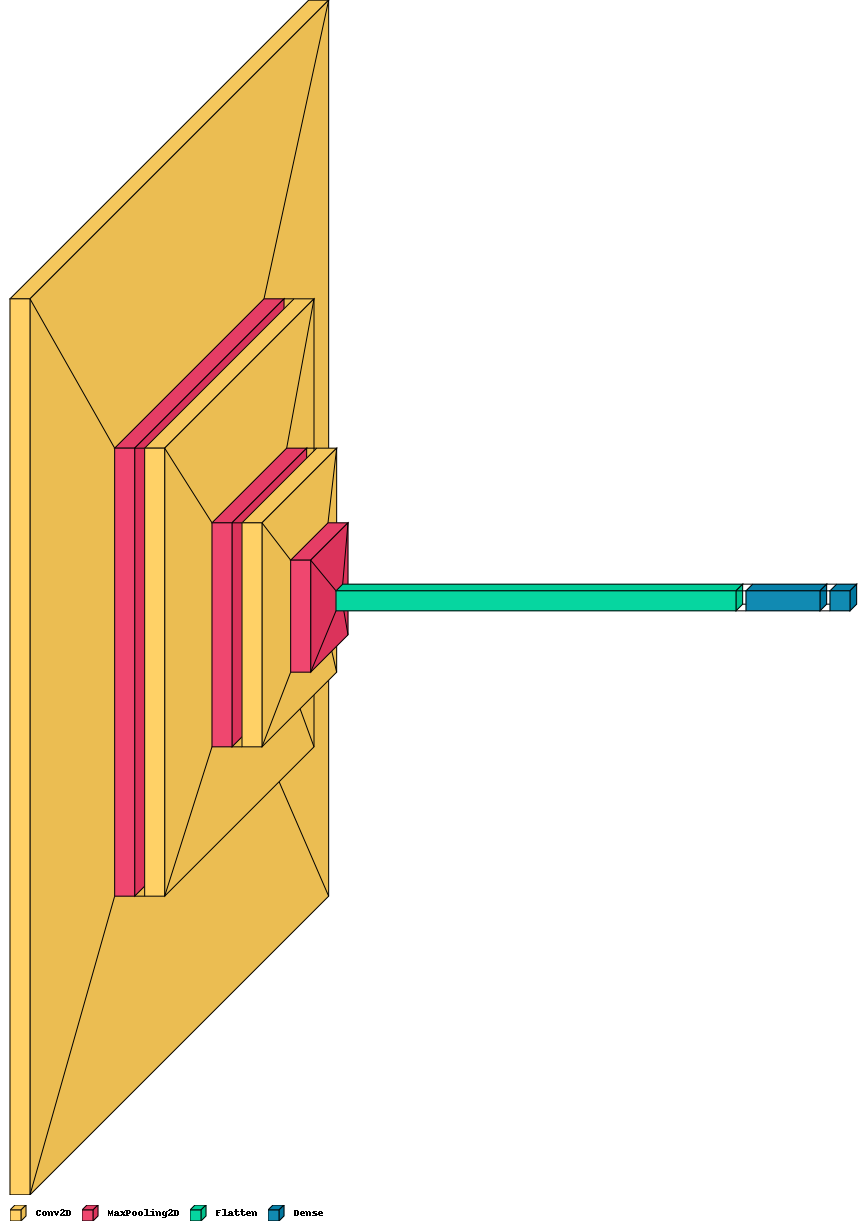
\includegraphics[width=0.85\linewidth]{schema.png}
  \caption{A schematic of the convolutional neural network}
  \label{schema}
\end{figure}

\noindent
In the Adam optimization algorithm, we seek to strike a balance between fast convergence and avoiding overshooting the optimal solution. The learning rate, denoted by $\alpha$, plays a crucial role in determining the step size taken during each update of the model's parameters. If $\alpha$ is too high, the algorithm might overshoot the optimal solution, leading to oscillations and instability in learning. On the other hand, if $\alpha$ is too low, the training process might become slow, requiring more iterations to reach convergence.

In our CNN model, we set a reasonable learning rate of $0.01$, as it has been found to be effective in many cases. However, the optimal learning rate can vary depending on the specific problem and model architecture. In practice, hyperparameter tuning techniques, such as learning rate scheduling and grid search, can be employed to find the best learning rate for a given task.

The loss function we use is the ``Categorical Cross Entropy'', which is well-suited for training a classification model with multiple classes. The Categorical Cross Entropy loss measures the dissimilarity between the predicted probabilities and the true one-hot encoded labels. By minimizing this loss, the model is encouraged to assign high probabilities to the correct class and low probabilities to the incorrect ones.

The concept of epochs is a fundamental aspect of the training process in machine learning. An epoch represents one complete iteration over the entire training dataset during the model training process. In our CNN model, we set the number of epochs to $10$. Each epoch takes approximately 10 minutes to run, making the overall training time reasonable. Selecting the right number of epochs is a crucial consideration. If we use too few epochs, the model may not have sufficient opportunities to learn and capture the underlying patterns in the training data, leading to underfitting. On the other hand, using too many epochs may result in overfitting, where the model becomes overly specialized to the training data and performs poorly on new, unseen data. Due to the long runtime required for each epoch, we did not explore increasing the number of epochs further. We also monitor the model's performance on a separate validation dataset and use a technique called early stopping to stop training once the model's performance on the validation data plateaus or starts to degrade, preventing overfitting and saving computational time. 

\section{Evaluation and Final Results} 
The plot of the loss and accuracy on the dataset is shown in Figure \ref{cnn_loss}. As observed, there is a notable difference between the training accuracy and validation accuracy, indicating the presence of overfitting. The model achieved a high training accuracy of 98.84\% but a lower validation accuracy of 82.84\%. To address the issue of overfitting and improve the model's overall performance, we apply two techniques: data augmentation and dropout.

\emph{1. Data Augmentation:}
   Data augmentation is a technique that involves generating additional training data by applying various transformations to the existing images. These transformations include flipping, rotation, shifting, and zooming. By augmenting the dataset with these variations, we introduce more diversity and variations to the training data, which helps the model generalize better to unseen images.

\emph{2. Dropout:}
   Dropout is a regularization technique that aims to reduce overfitting by randomly setting a fraction of the output units (neurons) to zero during training. This means that during each training iteration, a certain percentage of neurons are "dropped out" or deactivated, forcing the model to learn redundant representations and preventing complex co-adaptations between neurons. Dropout acts as a form of ensemble learning, as it trains multiple sub-networks with different combinations of neurons active and then averages their predictions during inference.

\noindent The dropout value used in the model was set to 0.2, meaning 20\% of the output units from the layer were randomly dropped out during training. The schematic of the Convolutional Neural Network with dropout is depicted in Figure \ref{dropout_schema}. This updated model with data augmentation and dropout shows improved generalization capabilities and better performance on unseen data.

\begin{figure}[htbp]
  \centering
  % Include the plot here using \includegraphics
  \caption{Plot of Loss and Accuracy on the Dataset}
  \label{cnn_loss}
\end{figure}

\begin{figure}[htbp]
  \centering
  % Include the dropout schematic here using \includegraphics
  \caption{Schematic of Convolutional Neural Network with Dropout}
  \label{dropout_schema}
\end{figure}

 \begin{figure}[h!]
 \centering
  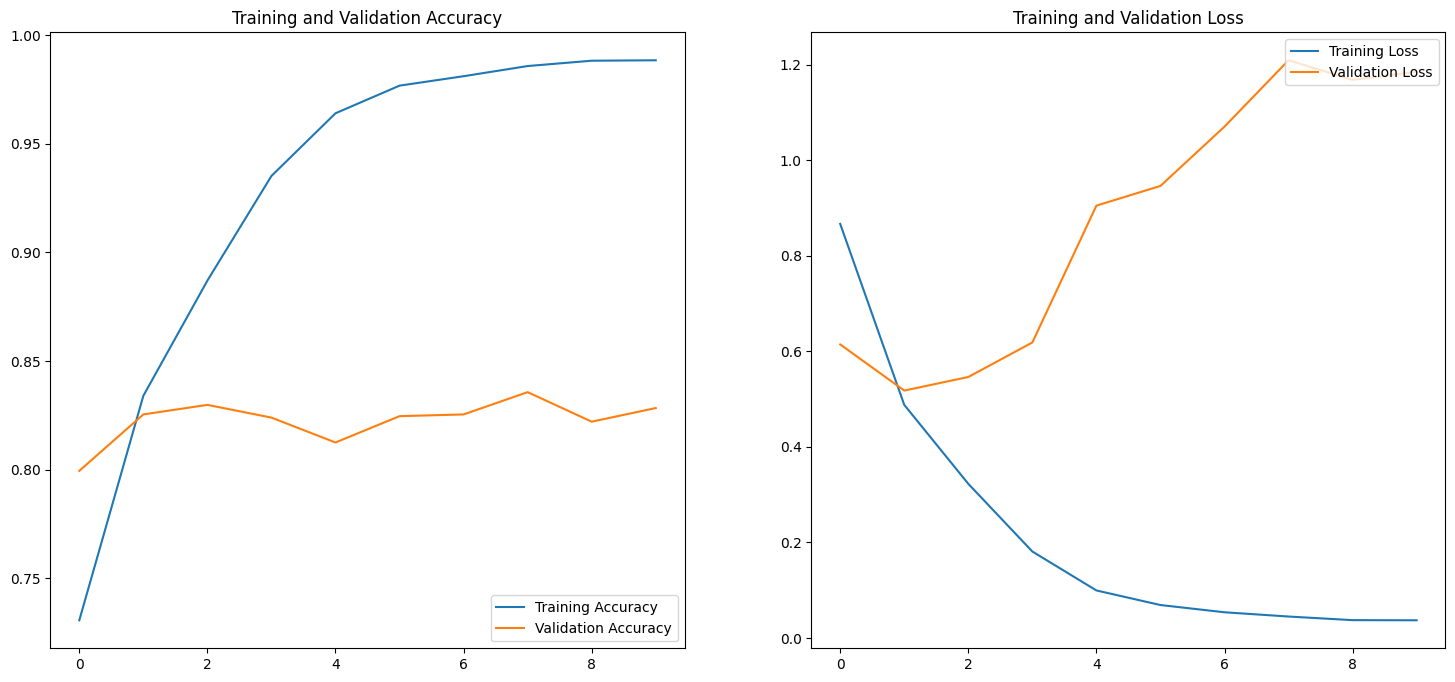
\includegraphics[width=\linewidth]{training_valid_plot.png}
  \caption{The Plot of Loss and Accuracy on Training Dataset}
  \label{cnn_loss}
\end{figure}

 \begin{figure}[h!]
 \centering
  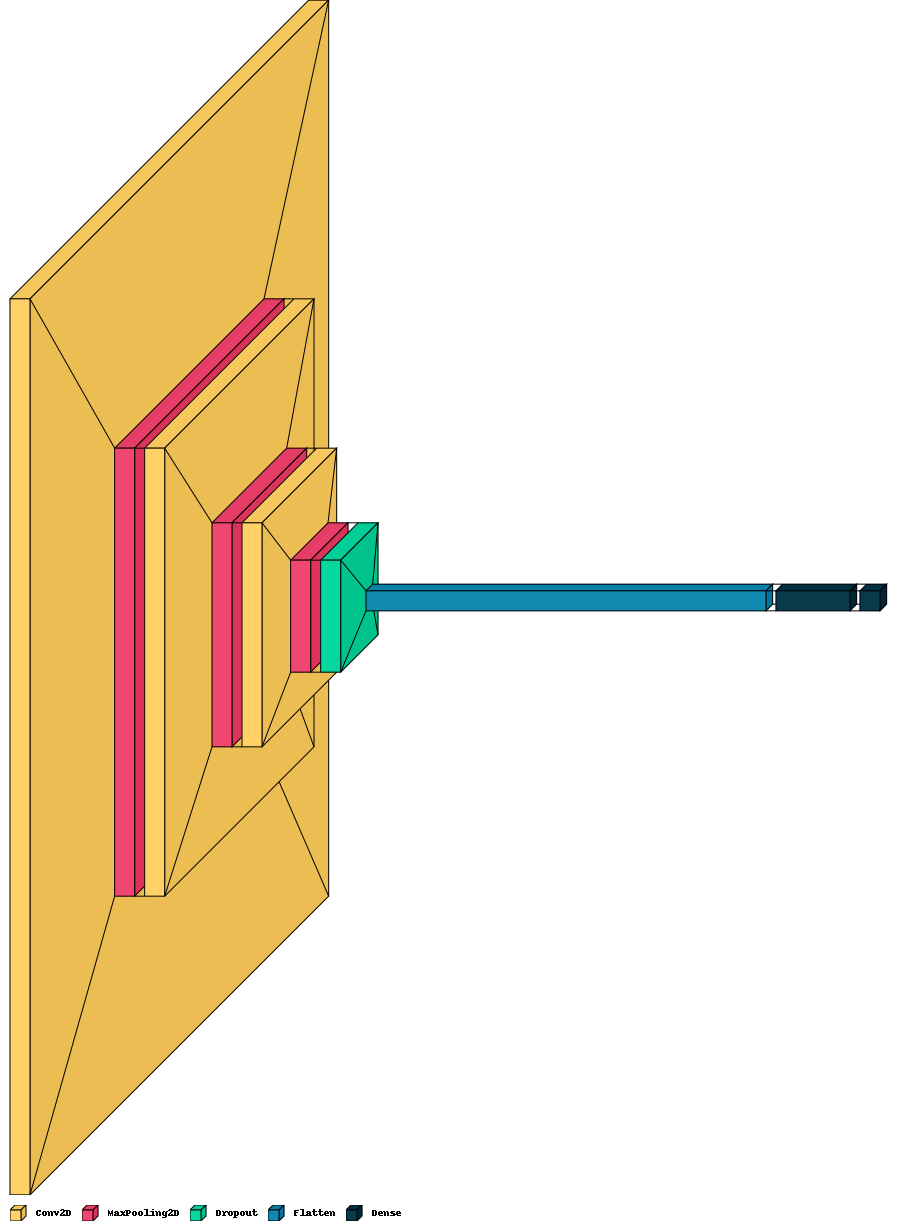
\includegraphics[width=0.85\linewidth]{dropout_schema.png}
  \caption{A Schematic of the Convolutional Neural Network with Dropout}
  \label{dropout_schema}
\end{figure}


 \begin{figure}[h!]
 \centering
  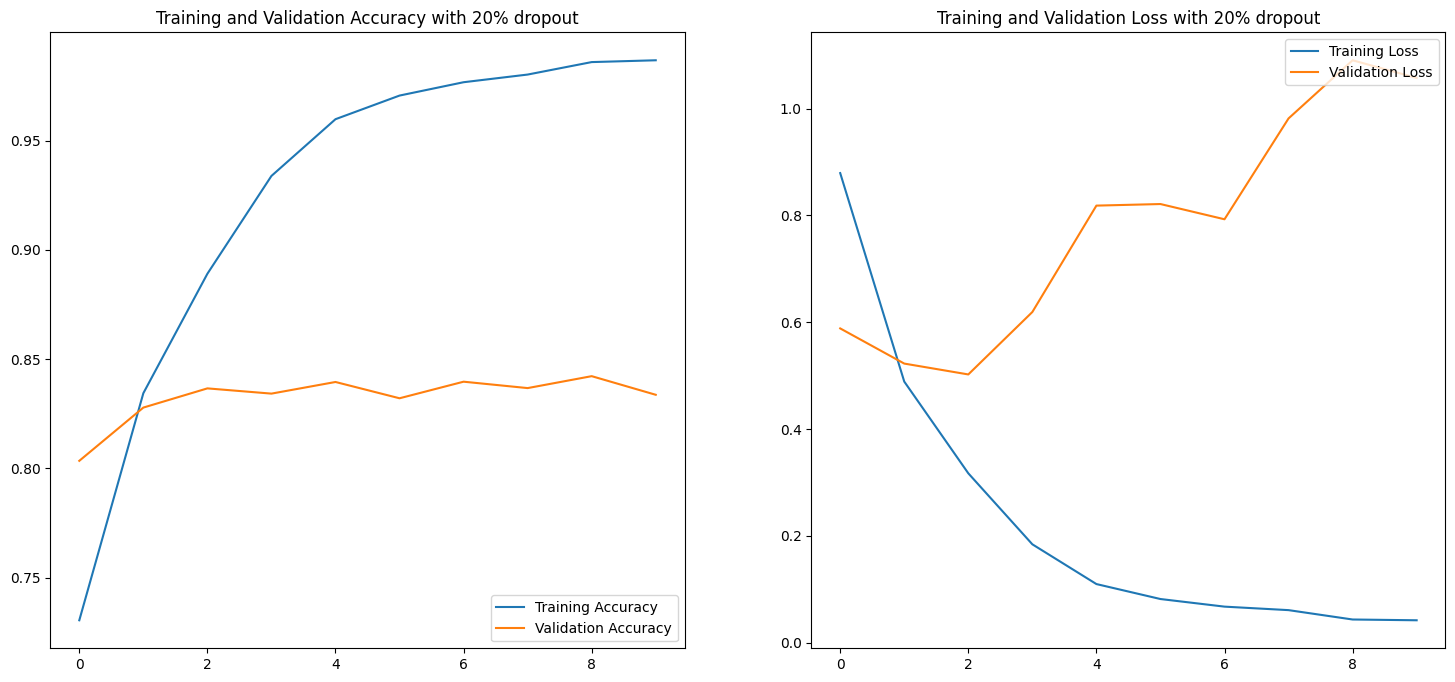
\includegraphics[width=\linewidth]{dropout_training_plot.png}
  \caption{The Plot of Loss and Accuracy on Training Dataset with Dropout}
  \label{dropout_training}
\end{figure}
\FloatBarrier

The plot of loss and accuracy on the training dataset with dropout is depicted in Figure \ref{dropout_training}. After training the model with dropout, we proceeded to make predictions on the test dataset to evaluate its performance. Before removing dropout, the model achieved an accuracy of 81.59\% on the test dataset. However, after removing 20\% dropout, the model's accuracy did not show any significant increase, reaching 98.68\%. On the other hand, the validation accuracy increased to 83.37\%, indicating that adding dropout did not lead to a noticeable improvement in model prediction.

One possible reason for not observing a significant improvement is that the original model already had a robust performance, and the dropout regularization might not have contributed significantly to its generalization. Additionally, with a large dataset and effective data augmentation techniques, the model might have been less prone to overfitting, making the impact of dropout less prominent.

Both models, with and without dropout, show the expected behavior during training: as the number of epochs increases, the loss decreases, and accuracy increases. This behavior is typical in the learning process of neural networks.

% Please add the following required packages to your document preamble:
% \usepackage{graphicx}
\begin{table}[h!]
\centering
\resizebox{\textwidth}{!}{%
Model Before Dropout
\begin{tabular}{lcccccccccc} \hline
Epoch                         & 1             & 2            & 3            & 4           & 5            & 6            &7            & 8           & 9           &10 \\
Loss                            & 0.8665 & 0.4879  & 0.3227  & 0.1810  & 0.0996  & 0.0690 & 0.0539 & 0.0450 & 0.0374 & 0.0371 \\
Train accuracy           & 0.7307  & 0.8340 & 0.8870  & 0.9352 & 0.9640  & 0.9768 & 0.9811   & 0.9858 & 0.9882 & 0.9884 \\
Validation accuracy   & 0.7995 & 0.8254  & 0.8298 & 0.8240 & 0.8125  & 0.8246 & 0.8254 & 0.8357 & 0.8221 & 0.8284 \\ \hline
\end{tabular}%
}
\caption{Result of Model Training and Validation Accuracy with Epochs}
\label{tab:train_loss}
\end{table}

% Please add the following required packages to your document preamble:
% \usepackage{graphicx}
\begin{table}[h!]
\centering
\resizebox{\textwidth}{!}{%
Model After Dropout
\begin{tabular}{lcccccccccc} \hline
Epoch                          & 1             & 2            & 3           & 4           & 5            & 6            &7            & 8            & 9            &10 \\
Loss                            & 0.8791   & 0.4889 & 0.3172 & 0.1843   & 0.1099  & 0.0819  & 0.0676 & 0.0611   & 0.0435  & 0.0421 \\
Train accuracy           & 0.7305  & 0.8344 & 0.8891 & 0.9339  & 0.9598  & 0.9706  & 0.9767 & 0.9803  & 0.9860  & 0.9868 \\
Validation accuracy   & 0.8035 & 0.8278 & 0.8366 & 0.8342 & 0.8395  & 0.8321 & 0.8397 & 0.8368 & 0.8422  & 0.8337 \\ \hline
\end{tabular}%
}
\caption{Result of Model Training and Validation Accuracy After Dropout with Epochs}
\label{tab:dropout_train_loss}
\end{table}

To further re-fine the model, we increased the number of dense layers of the CNN model with two additional layers: one with 512 units and one with 256 units. Looking at Table 3, there is not much difference in the training accuracy nor validation accuracy between the refined model and the previous two models, and both accuracies seem to be close to the previous models. Moreover, the training and validation accuracy even is lower at around 81\%, and so serves as an indicator that adding additional layers to this model might be overfitting the data and might not be neccessary, causing the decreased accuracies.
 
  \begin{figure}[h!]
 \centering
  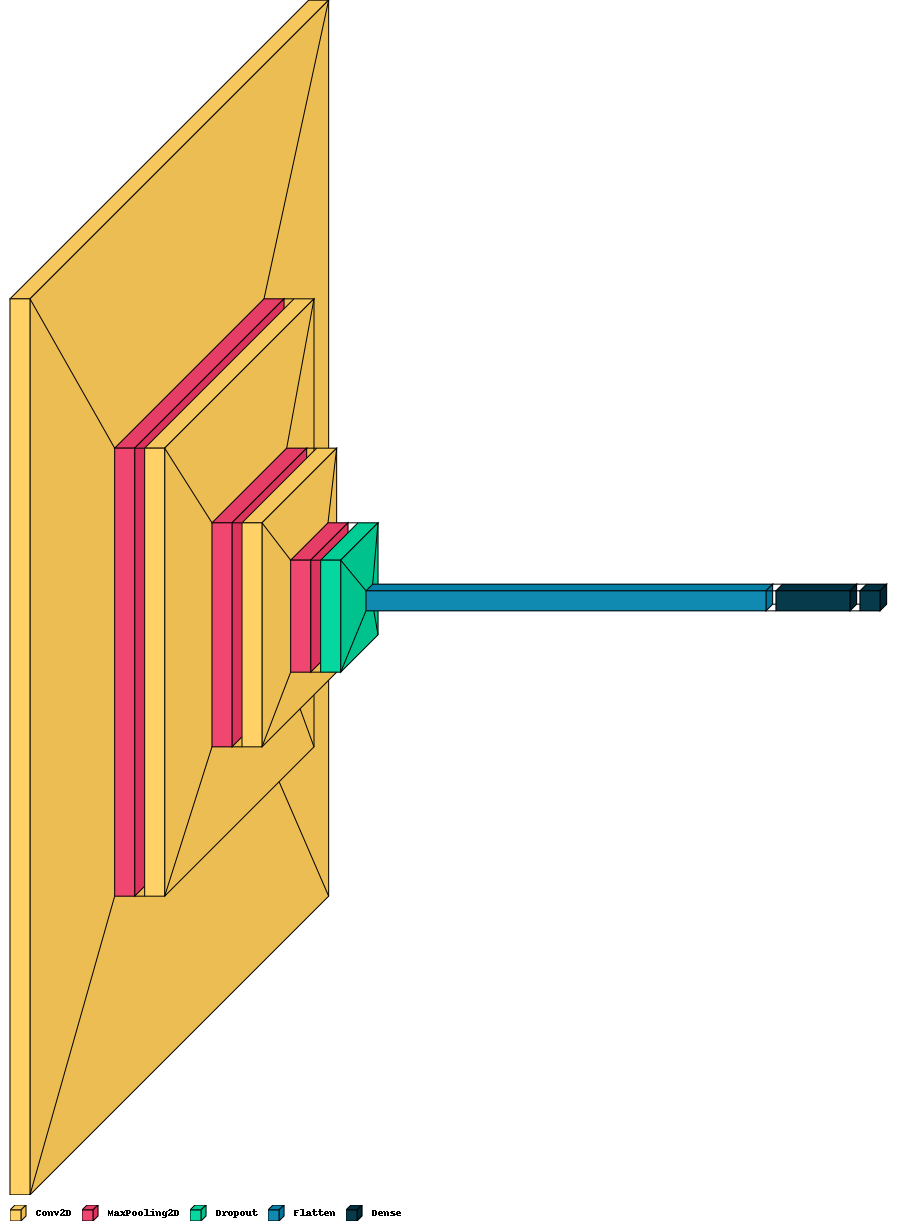
\includegraphics[width=0.85\linewidth]{refined_schema.png}
  \caption{A Schematic of the Convolutional Neural Network with Additional Layers}
  \label{refined_schema}
\end{figure}
 
 \begin{figure}[h!]
 \centering
  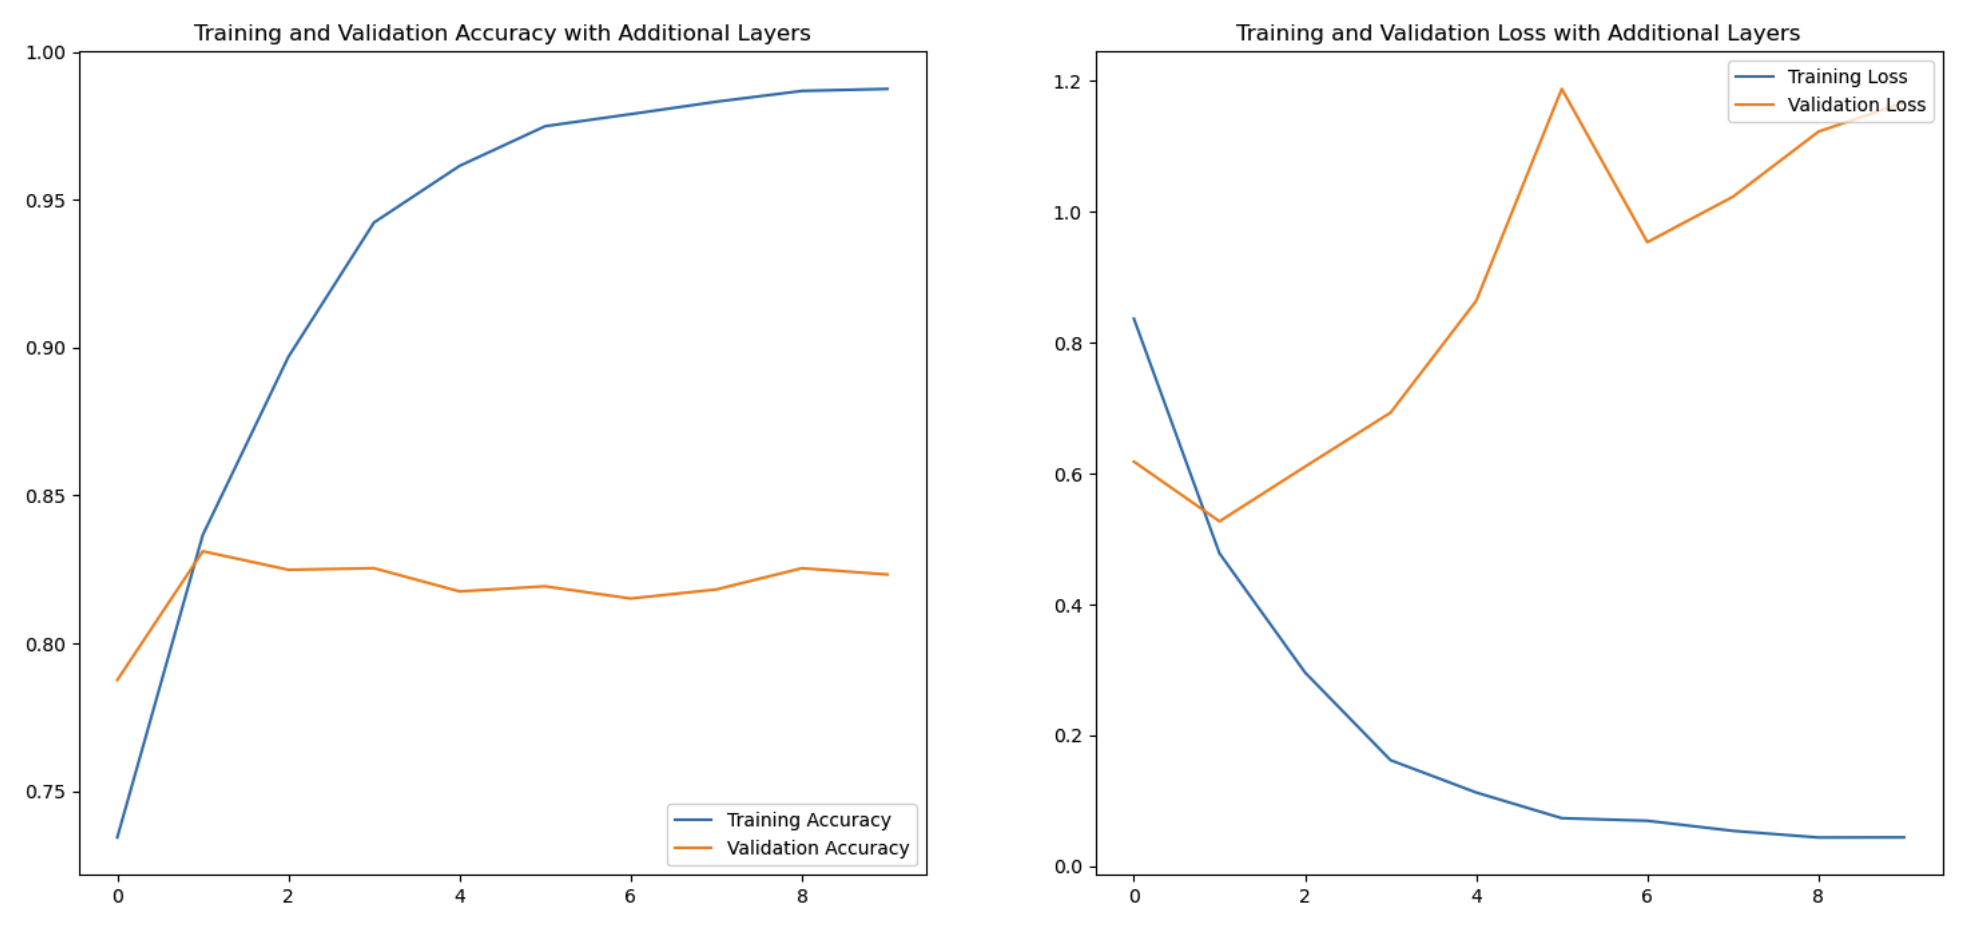
\includegraphics[width=\linewidth]{Model with Additional Layers.png}
  \caption{The Plot of Loss and Accuracy on Training Dataset with Additional layers}
  \label{refined_model_training}
\end{figure}
\FloatBarrier

% Please add the following required packages to your document preamble:
% \usepackage{graphicx}
\begin{table}[h!]
\centering
\resizebox{\textwidth}{!}{%
Refined Model with Additional Layers
\begin{tabular}{lcccccccccc} \hline
Epoch                         & 1             & 2            & 3           & 4           & 5            & 6           &7            & 8            & 9           &10 \\
Loss                           & 0.8664 & 0.4981   & 0.3190   & 0.2033 & 0.1274 & 0.0955 & 0.0702 & 0.0586 & 0.0612 & 0.0487\\
Train accuracy          & 0.7238 & 0.8331   & 0.8887 & 0.9291 & 0.9567   & 0.9676 & 0.9766& 0.9820  & 0.9809  & 0.9862\\
Validation accuracy  & 0.7909 & 0.8193   & 0.8144 & 0.8286 & 0.8197 & 0.8197 & 0.8352 & 0.8148 & 0.8288 & 0.8197\\ \hline
\end{tabular}%
}
\caption{Result of Model Training and Validation Accuracy After Additional Layers with Epochs}
\label{tab:refined_train_loss}
\end{table}

Furthermore, we evaluated the model's performance on the designated test dataset, and the accuracy achieved was an 82.7\%, indicating the model's capability to generalize well to new and diverse shoe images.

\section{Conclusion}
In conclusion, our Convolutional Neural Network (CNN) model has demonstrated impressive accuracy in correctly identifying shoe classes from images, laying a strong foundation for future advancements in image classification that can significantly enhance consumer-driven shopping experiences. The success of CNN models in image classification makes them a versatile and powerful tool for various applications.


\noindent While our model achieved high accuracy, we acknowledge that further improvements would involve comparing its performance with other well-known pre-trained models like ResNet50 and Fastai. Additionally, more sophisticated optimization algorithms, learning rate schedulers, and regularization techniques can be employed to fine-tune the model's training process and achieve better performance. Such a comparison can provide valuable insights into the strengths and weaknesses of different approaches to image classification. Another area for improvement is to increase the dataset size. By adding more diverse images of shoes with different backgrounds and including additional objects in the images, we can train the model to recognize and classify images more intelligently. This would improve the model's ability to generalize to new, unseen data and enhance its accuracy in real-world scenarios.

\noindent Looking ahead, we envision deploying the trained model as a user-facing application to deliver a seamless and user-friendly shopping experience. By allowing consumers to upload images and receive the corresponding shoe model names as output, this application can drastically simplify the process of identifying and purchasing specific shoe models, elevating customer satisfaction and engagement. The potential of integrating our image classification system into popular platforms, such as Instagram or a web application, holds tremendous benefits for retailers and e-commerce platforms. By incorporating this product identification feature, businesses can captivate potential buyers, drive conversions, and maximize sales potential. This transformative capability effectively bridges the gap between inspiration and purchase, transforming social media platforms into powerful sales channels.

\pagebreak
\section{References} 
		\begin{enumerate}
		\item Albawi, S., Mohammed, T. A., \& Al-Zawi, S. (2017). Understanding of a Convolutional Neural Network. 2017 International Conference on Engineering and Technology (ICET), 1–6. https://doi.org/10.1109/icengtechnol.2017.8308186
		
		\item Sharma, N., Jain, V., \& Mishra, A. (2018). An Analysis Of Convolutional Neural Networks For Image Classification. Procedia Computer Science, 132, 377–384. https://doi.org/10.1016/j.procs.2018.05.198
		\item Yu, A., \& Grauman, K. (2014). Fine-Grained Visual Comparisons with Local Learning. Computer Vision and Pattern Recognition. https://doi.org/10.1109/cvpr.2014.32 
		\end{enumerate}
\end{document}